% Options for packages loaded elsewhere
\PassOptionsToPackage{unicode}{hyperref}
\PassOptionsToPackage{hyphens}{url}
%
\documentclass[
]{book}
\usepackage{lmodern}
\usepackage{amssymb,amsmath}
\usepackage{ifxetex,ifluatex}
\ifnum 0\ifxetex 1\fi\ifluatex 1\fi=0 % if pdftex
  \usepackage[T1]{fontenc}
  \usepackage[utf8]{inputenc}
  \usepackage{textcomp} % provide euro and other symbols
\else % if luatex or xetex
  \usepackage{unicode-math}
  \defaultfontfeatures{Scale=MatchLowercase}
  \defaultfontfeatures[\rmfamily]{Ligatures=TeX,Scale=1}
\fi
% Use upquote if available, for straight quotes in verbatim environments
\IfFileExists{upquote.sty}{\usepackage{upquote}}{}
\IfFileExists{microtype.sty}{% use microtype if available
  \usepackage[]{microtype}
  \UseMicrotypeSet[protrusion]{basicmath} % disable protrusion for tt fonts
}{}
\makeatletter
\@ifundefined{KOMAClassName}{% if non-KOMA class
  \IfFileExists{parskip.sty}{%
    \usepackage{parskip}
  }{% else
    \setlength{\parindent}{0pt}
    \setlength{\parskip}{6pt plus 2pt minus 1pt}}
}{% if KOMA class
  \KOMAoptions{parskip=half}}
\makeatother
\usepackage{xcolor}
\IfFileExists{xurl.sty}{\usepackage{xurl}}{} % add URL line breaks if available
\IfFileExists{bookmark.sty}{\usepackage{bookmark}}{\usepackage{hyperref}}
\hypersetup{
  pdftitle={Data Ethics, AI and Responsible Innovation},
  pdfauthor={Nick Hood},
  hidelinks,
  pdfcreator={LaTeX via pandoc}}
\urlstyle{same} % disable monospaced font for URLs
\usepackage{longtable,booktabs}
% Correct order of tables after \paragraph or \subparagraph
\usepackage{etoolbox}
\makeatletter
\patchcmd\longtable{\par}{\if@noskipsec\mbox{}\fi\par}{}{}
\makeatother
% Allow footnotes in longtable head/foot
\IfFileExists{footnotehyper.sty}{\usepackage{footnotehyper}}{\usepackage{footnote}}
\makesavenoteenv{longtable}
\usepackage{graphicx}
\makeatletter
\def\maxwidth{\ifdim\Gin@nat@width>\linewidth\linewidth\else\Gin@nat@width\fi}
\def\maxheight{\ifdim\Gin@nat@height>\textheight\textheight\else\Gin@nat@height\fi}
\makeatother
% Scale images if necessary, so that they will not overflow the page
% margins by default, and it is still possible to overwrite the defaults
% using explicit options in \includegraphics[width, height, ...]{}
\setkeys{Gin}{width=\maxwidth,height=\maxheight,keepaspectratio}
% Set default figure placement to htbp
\makeatletter
\def\fps@figure{htbp}
\makeatother
\setlength{\emergencystretch}{3em} % prevent overfull lines
\providecommand{\tightlist}{%
  \setlength{\itemsep}{0pt}\setlength{\parskip}{0pt}}
\setcounter{secnumdepth}{-\maxdimen} % remove section numbering
\usepackage{booktabs}
\usepackage{amsthm}
\makeatletter
\def\thm@space@setup{%
  \thm@preskip=8pt plus 2pt minus 4pt
  \thm@postskip=\thm@preskip
}
\makeatother
\AtBeginDocument{\renewcommand{\chaptername}{Week}}
\newlength{\cslhangindent}
\setlength{\cslhangindent}{1.5em}
\newenvironment{cslreferences}%
  {\setlength{\parindent}{0pt}%
  \everypar{\setlength{\hangindent}{\cslhangindent}}\ignorespaces}%
  {\par}

\title{Data Ethics, AI and Responsible Innovation}
\author{Nick Hood}
\date{24 November 2020}

\begin{document}
\maketitle

{
\setcounter{tocdepth}{0}
\tableofcontents
}
\hypertarget{introduction}{%
\chapter*{Introduction}\label{introduction}}
\addcontentsline{toc}{chapter}{Introduction}

These are my notes from participation in the Edinburgh Data Ethics MOOC, running in November and December 2020. Any errors here are my own responsibility.

Nick Hood\\
\href{https://twitter.com/NixImagery}{@NixImagery}

This document was last updated on 24 November 2020 at 09:23.

\hypertarget{course-overview}{%
\section*{Course overview}\label{course-overview}}
\addcontentsline{toc}{section}{Course overview}

\begin{description}
\tightlist
\item[Week 1 Ethics and Law]
What are ethical values? Can we rely on legal regulation? What are the most pressing issues facing data driven industries?
\item[Week 2 Crime and Justice]
Should we use predictive policing and sentencing algorithms? How can biases sneak into such algorithms? How can we remove them?
\item[Week 3 Home and City]
What are the promises of smart homes and cities? How can they impact our privacy and freedom? How can we design them to protect those values?
\item[Week 4 Money and Markets]
Can future tech lead to a world without money? Can algorithms help us fairly distribute resources? How could we design a fair AI?
\item[Week 5 Life and Health]
Should we keep genetic databanks? Would you trust an AI doctor? What are the principles of responsible research and innovation?
\end{description}

\hypertarget{week-1-ethics-and-law}{%
\chapter{Week 1: Ethics and Law}\label{week-1-ethics-and-law}}

This starts with some housekeeping, introductions to the tutors and setting up a profile within the course. Dr.~Ewa Luger gets us started by considering a ``broad overview'' of \textbf{ethics}, using a radio interview about the Cambridge Analytica (CA) scandal as a resource to get us thinking before we embark on a more detailed introduction to ethics.

\begin{itemize}
\tightlist
\item
  Ethical `Issues'
\item
  Introduction to Ethics
\item
  Legal and ethical Considerations
\item
  Information, Control and Power
\end{itemize}

\hypertarget{ethical-issues}{%
\subsection{Ethical `Issues'}\label{ethical-issues}}

In the clip, problematised issues with the CA matter included:

\begin{itemize}
\tightlist
\item
  the way data was gathered from people
\item
  the fact that the data was then passed on to another party
\item
  that the data was now available for commercial use
\item
  that the data was used for political purpose
\item
  the FaceBook (FB) login on an app gave permissions for all of users' FB data to be used and shared
\item
  people aren't outraged, or even bothered by this enough to take action
\end{itemize}

\begin{description}
\tightlist
\item[Discussion forum task]
Think back over your professional life and identify one example of an ethical issue that you personally experienced. In the discussion forum, write a brief summary (around 50-100 words) describing this issue - try to explain the context, what happened, and why you felt it was an ethical issue. After you've done this, comment on two other posts.
\end{description}

I had to take a quick look at the forum first to gauge the level of ethical matters that were being shared. There seems to be a discernible difference between \textbf{moral}, \textbf{legal} and \textbf{ethical} matters in the revelations on the forum. My own example came from quite a selection of professional experience that ranged from legal but immoral, moral but illegal, unethical but moral and legal. I picked an example from a while back.

\begin{quote}
I was project manager in a business that made flight crew training simulators. These devices were multi-million-dollar complex machines that used specially designed and manufactured circuit boards mounted in standard racks to drive the various components of the device. I had an internal review one morning that failed badly when the equipment that had been working well the night before suddenly failed to function. It was extremely embarrassing for my team. We discovered later that day that in the night, another project manager had switched a key circuit board for a faulty one from his own machine.
\end{quote}

The other examples I commented on or read seemed to me to be not so much ethical issues as difficult choices or situations. This is causing me to wonder if I have a secure understanding of the term, ``ethical''. Hopefully the next section will clear that up for me.

\hypertarget{the-challenge-of-data-driven-innovation}{%
\section{The challenge of data-driven innovation}\label{the-challenge-of-data-driven-innovation}}

Issues arising from the 2018 Cambridge Analaytica scandal are identified as:

\begin{itemize}
\tightlist
\item
  the value derived from data is not evenly distributed
\item
  power rests in the hands of very few
\item
  the potential for harm and inequality is high
\item
  the potential impact of bad actors
\end{itemize}

These are, in my view, issues of power arising from wealth inequity and not particularly related to anything technological. The difficulty is that technology amplifies the effects (as it amplifies inequities in a classroom -- this much we have learned in moving to ``Digital First'' pedagogies resulting from the COVID measures).

The basic principles of ethics are described as, ``how we should address these issues, whilst minimising harm, ensuring morally good outcomes and fairness, and protecting human autonomy.''

\hypertarget{data-at-the-heart-of-it}{%
\subsection{Data at the heart of it}\label{data-at-the-heart-of-it}}

For the purposes of the course, this definition of ethics is set in the context of \emph{data-driven innovation} which makes use of large amounts of data to train algorithms that make predictions or provide insights for decision making. Machines are increasingly now involved in the decision making too, and in taking actions. These machines are described as \emph{intelligent}.

\hypertarget{visibility-of-rationale}{%
\subsection{Visibility of rationale}\label{visibility-of-rationale}}

These machines include, of course, neural networks and we know from the way that these pattern-matchers work, that other than the input and output layers, it is not possible to determine the path of the rationale -- the specific choices ot selections being made in the intermediate steps -- that underlies the outputs.

\hypertarget{ambient-intelligent-systems}{%
\subsection{Ambient intelligent systems}\label{ambient-intelligent-systems}}

Interactional moments are perceived to provide friction in the operation of systems, therefore designers are removing these for a smoother experience -- think of entering your password every time you wanted to look at your phone, now replaced with fingerprint or face recognition. The result is that such interactions become invisible to the user: it is the environment we interact with in a natural way. Unnaturally, \emph{the environment is reading us to discern intent}.

\hypertarget{human-ai-interaction}{%
\subsection{Human --\textgreater{} AI interaction}\label{human-ai-interaction}}

This is problematised in a video clip, suggesting that this interaction is not yet defined. I rather think that Turing (\protect\hyperlink{ref-TURING1950}{1950}) had a clear enough view of what it might look like, but recent innovations have increased \emph{system opacity} such that understanding how the system makes choices based upon how it perceives us is difficult. In some sense, we are already familiar with this idea with our less tech-savvy relatives who need support working with machines. It gets harder when you don't know there's a machine.

\hypertarget{utility}{%
\subsection{Utility}\label{utility}}

Comparison with basic utilities like water, power, etc., is made from a very privileged first-world perspective: \emph{we only notice them when they fail}. These systems were unregulated in their early days, too, and some of the horrors of human behaviour (Edison, for example) are long forgotten. As data-driven innovation moves to infect our lives by becoming a utility, the question is asked, ``should it be regulated?'' First steps have been made in this, of course, and we see the return of interactional friction with things like the cookie quiz on GDPR-compliant websites. The monetisation of data has led to the term, ``surveillance capitalism'', which describes how our identity and behaviours have become the product in a high-value industry.

\hypertarget{policy-lag}{%
\subsection{Policy lag}\label{policy-lag}}

Clearly, policy makers are well behind the curve when it comes to data-driven innovation. GDPR and similar legislation have added friction yet advances are made at speed. The additional reading (Wagner, \protect\hyperlink{ref-Hildebrandt2019}{2019}) is critical of policy makers and suggests that ethics is what corporations do to avoid government interference.

\hypertarget{values}{%
\subsection{Values}\label{values}}

What we value in society is a cultural attribute. Values are therefore dependent on context and are not absolute: I have often said that every principle has a price attached to it, and that if the price is right, all principles are for sale. This has caused strong reaction when vocalised that way, especially from those who feel that they themselves hold high principles in comparison with others. Clearly, passions are aroused when deeply-held values are challenged, as the \href{https://www.theguardian.com/lifeandstyle/1999/nov/06/weekend.kevintoolis}{Guardian article on Peter Seeger} illustrates.

Examples are discussed in the course material to illustrate the point that values depend very much on context. This statement is a call to action, perhaps, talking of moral dilemmas and conflicting values:

\begin{quote}
``Our job, as ethical actors, is to identify what they are, and then negotiate how best to instantiate and balance them.''
\end{quote}

Research is as robust as you'd expect for the social sciences, with this, from a study of a small sample of people (N \textless{} 700) in three countries with similar (colonial) cultural pedigree:

\begin{quote}
``\ldots{} people endorse the same values to a similar extent across countries and also instantiate them similarly.'' (Bardi et al., \protect\hyperlink{ref-Bardi2018}{2018})
\end{quote}

Not much of a surprise there, given the evolutionary path of the handful of people studied.

\hypertarget{case-studies}{%
\subsection{Case studies}\label{case-studies}}

Proejct Maven and the Google employee revolt against it is presented as the first case study of how corporations can make choices that do not align with the values of the stakeholders, in this case, the staff. That project sat in stark contrast to Google's \href{https://en.wikipedia.org/wiki/Don\%27t_be_evil}{``Don't be evil''} mantra, still enshrined in its code of conduct (cf.~the characterisation of ethics as an escape from regulation by Wagner (\protect\hyperlink{ref-Hildebrandt2019}{2019})). The military application of data-driven innovation is clearly compelling, and others are emerging, including \href{https://www.nytimes.com/2020/01/18/technology/clearview-privacy-facial-recognition.html}{Clearview AI's face recognition app}, which \href{https://clearview.ai/}{the company} has worked hard to present as ethical use of technology.

\hypertarget{what-are-ethics}{%
\section{What are ethics?}\label{what-are-ethics}}

A branch of moral philosophy: a codification of habits that are valued within the context of a culture: ergo, no right or wrong answers, just human custom. \emph{Normative} ethics are those that define what we \emph{ought} to do, without concerning themselves with what we \emph{actually} do. Within that class of ethics are 3 persepctives on how we should act:

\begin{description}
\tightlist
\item[Deontological ethics (rules)]
rules of duty and obligation -- perhaps universally agreed upon, like not killing each other, or hurting animals. Some things are always right, others, always wrong, no matter the consequences.
\item[Teleological ethics (consequences)]
focus on the outcome of actions -- actions for the greater good, perhaps, or the end justifying the means. \emph{Consequentialism} is the view that the moral quality of a choice is decided solely by its outcome.
\item[Virtue ethics]
are about judgement of people's character or moral fibre.
\end{description}

The obvious issue here is that life is complicated, isn't it? We can't make a simple set of rules because the complexity of life requires us to make choices sometimes that go against those simple rules for a better end. Is there any point, then, in having rules in the first place? Well, clearly, because we want everyone else to make choices that don't harm or disadvantage us.

\hypertarget{the-trolley-problem}{%
\subsection{The trolley problem}\label{the-trolley-problem}}

\begin{description}
\tightlist
\item[Scenario 1]
A runaway train is travelling on a railway track towards 5 people. You can't warn them, but there is a lever that you can operate to switch the tracks. The problem is that there is a person on the other track. \textbf{Do you pull the lever or not?}
\item[Scenario 2]
As above, but now there are no points -- instead, a large person standing a bridge over the tracks. \textbf{Do you push Fatty into the path of the train to save the five?}
\end{description}

I chose yes in both scenarios.

\begin{quote}
``The needs of the many outweigh the needs of the few.'' -- Spock
\end{quote}

Interestingly, although I was with the majority in the first scenario, I was in the minority in the second. I don't understand this difference, except for the difference between operating a control like the lever, and physically acting on another human being -- the former seems less connected to the action, perhaps.

\begin{description}
\tightlist
\item[Other scenarios]
How does the trolley problem change when the 5 are convicted rapists? Children? When Fatty is a scientist working on a cure for Leukemia? When the 5 are Mountain People (insert your own other-class of person)? Tories? Welsh? Rednecks?
\end{description}

\hypertarget{making-moral-decisions}{%
\subsection{Making moral decisions}\label{making-moral-decisions}}

So, are ethics about choices, or outcomes? Rules or consequences?

MIT are trying to build a picture of moral acceptability with their crowdsourcing \href{https://www.moralmachine.net/}{moral machine} project in which you are presented with multiple scenarios (like driverless car choices) in which you decide the path the vehicle should take, usually resulting in somebody or something dying. It is easy to become quickly abstracted from the awfulness of the choices you make in this game.

Guidelines in ethical frameworks for machine choices are broadly divided into four categories:

\begin{itemize}
\tightlist
\item
  Do good
\item
  Minimise harm
\item
  Respect human autonomy
\item
  Be just or fair
\end{itemize}

Someone should tell Peugeot about the third one. My wife's 2008 has a really irritating habit of grabbing the wheel if you change lanes without indicating, thinking that you've fallen asleep. I haven't found a way of switching that off yet, but it is really disconcerting, especially on a long trip at night with no other vehicles around.

Transparency of the algorithm and accountability are increasingly being emphasised. These frameworks have become regarded as inadequate as they offer a way for corporations to hide behind them in what is called, ``ethics washing''. This is a problem for all rules or specifications, or checklists.

\hypertarget{decision-making-in-scottish-teacher-education}{%
\subsubsection{Decision-making in Scottish Teacher Education}\label{decision-making-in-scottish-teacher-education}}

In my own application, teacher education\footnote{We don't like ``teacher training'' because we like to think that teaching is a profession, like the law, or the military. It isn't, of course, but we sustain the pretence for ourselves, even if nobody else in society beleives it.}, the \href{https://www.gtcs.org.uk/professional-standards/standards-for-registration.aspx}{GTCS Professional Standards} are meant to provide an objective benchmark that describes the competencies and skills of all teachers in Scotland. We know that the application of these standards is in the hands of the profession itself and therefore wildly variable in their interpretation. The standards themselves are written in ambiguous and wishy-washy language, like most things in state-provisioned education, and so are highly subjective and open to -- interpretation or abuse, depending on your view of an individual situation.

\begin{quote}
``\emph{Universal law is for lackeys. Context is for kings.}'' --Lorca (Goldsman, \protect\hyperlink{ref-Goldsman2019}{2019})
\end{quote}

\hypertarget{moral-decision-making-applied-to-data-ethics}{%
\subsubsection{Moral decision-making applied to data ethics}\label{moral-decision-making-applied-to-data-ethics}}

A couple of questions are asked in a section making the links between moral decision making and data ethics. The first, ``\emph{Should we require people to give their DNA to a gene bank?}'', screams at me, perhaps because of my age and the closeness people of my age have, although not by first-hand experience, of the horrors of the Second World War. Everything about centralised reporting of ethnicity makes me recoil: I never provide information about my ethnicity, and I would need a very good reason before I ever did. We are forgetting: something that gets me in trouble almost every year, with very real regret and a deepening sense of injustice\footnote{When I call people out for their disrepect of the remembrance observation, it is always me that is critiqued for not being kind, or collegiate. People can be so ungrateful and selfish. The injustice of such treatment makes me wonder.}.

The second question relates to social media and their handling of ``hate speech''. This is topical: I have just deleted my personal Facebook account\footnote{I am keeping, uncomfortably, a couple of social media accounts going that are related to my media and technical interests. Incidentally, I also deleted my personal Twitter account, but not for this reason. I'm generally a bit fed up with the whole Internet at the moment.} after they, once again, dismissed my objections to posts intended to whip up hatred of muslims, or other racial or ethnic groupings. In every case I have raised, the posts have not been found to breach codes of conduct, illustrating what is described as ethical washing (see above). To my cost -- I have cut off friends and family with whom I am only connected this way -- I have deleted my account.

\hypertarget{a-thought-experiment}{%
\subsection{A thought experiment}\label{a-thought-experiment}}

We are tasked with making our own thought experiment to allow us to examine our beliefs and ``surface'' factors that influence our judgement. This is mine.

\begin{description}
\item[The question]
Is it OK to kill to save lives in a war when you are not a combatant?
\item[Parameters]
In the context of war, it is given that the combatants of one side are allowed to kill the combatants of the other. What constitutes ``combatant'', however? Is it anyone who wears the uniform, or stands behind the barricades? What about observers?
\item[The story]
During an African war, a soldier of an impartial peacekeeping force (soldier A) is invited to take a ride in a helicopter on a routine supply drop to a station in the bush. Soldier A has not been explicitly told that he is not allowed to ride in the vehicles of either side. The route is a well-known safe corridor, well policed by peacekeepers and respected by both sides in the war. Soldier A takes the ride, seated in the open side door of the helicopter next to a mounted cannon. En route, the helicopter comes under fire unexpectedly. The pilot takes evasive action by banking sharply to right. Soldier A can see smoke coming from a group of boulders on the ground directly below him. He realises that his life, and the lives of the others in the helicopter are in danger. He hears the pilot on the intercom shouting, ``Shoot them! Shoot them!''

\textbf{You are soldier A. Do you use the cannon and try to save yourself and the crew?}
\end{description}

\hypertarget{legal-and-ethical-considerations}{%
\section{Legal and ethical considerations}\label{legal-and-ethical-considerations}}

\hypertarget{legal}{%
\subsection{Legal}\label{legal}}

Well, let's not pretend that there's much of a connection between law and morality. Laws are instruments of power. They belong to the powerful. Even at mate's rates, a lawyer's fees are vulgar and shameless. Even if it were accessible by the common people, legal decisions have always been historically hysterical, wildly inconsistent and woefully inadequate. It's noticeable that the great democratisers of the law have been people like Napolen and Hitler. It's about time we replaced the whole system with a machine.

\begin{quote}
``\emph{The first thing we do, let's kill all the lawyers.}'' -- Henry VI, Part 2, Act IV, Scene 2 (\protect\hyperlink{ref-Shakespeare}{1591})
\end{quote}

The laws of the land are the first and greatest example of what the course describes as ``ethics washing'', the practice of corporations who create ``codes'' to \emph{lure the public into a false sense of security and earn undeserved trust}. Laws make us feel safe but do nothing to make us safe as enforcement and monitoring are lacking.

In the same way that the discussion in the course speaks of ethics guidelines being used by companies ``to ward off regulation by the state through formal laws'', so government uses laws to ward off revolution and disorder.

There is a tension in data ethics between the need and cost of self-regulatory codes of conduct, and external regulation through the courts. The course summarises data ethics and the law:

\begin{description}
\tightlist
\item[Hard ethics]
is needed to understand and interpret laws, and to make sure legislation is followed.
\item[Soft ethics]
are normative rules that tell us how to behave morally, whether the law addresses our actions or context.
\item[Compliance with the law]
is normally necessary for ethically correct conduct, but may not be enough for it.
\end{description}

\hypertarget{ethical-nothing-ethical-going-on-here.}{%
\subsection{Ethical? Nothing ethical going on here.}\label{ethical-nothing-ethical-going-on-here.}}

I skimmed the transcript of the role-play presented by the course (I am out of week already) and also the discussion on the ethics of setting cookies for the participants of ths MOOC. Much angst, I see.

Tracking is an issue for me and therefore I take steps to mitigate it. I don't allow setting of third-party cookies, and have a policy of clearing all cookies on exit from a browser session. I also use different browsers. Tracking is difficult under those circumstances: this is working for me. How do I know? When I get advertising, it's usually totally irrelevant, which gives me some comfort, but I'm not complacent about it. I hate advertising: it's one of the manifestations of what is truly awful about human beings.

Solutions like the GDPR persmissions dialogues are no better than the advertising itself. They doesn't solve any problems, they just get in the way and decrease the chances of me using the sites that push them into my face. I make use of ad blockers, brutal cookie policy, and text readers when using the web.

Interestingly, the link to the EC directive yields a 404 (not found) error. The \href{https://support.edx.org/hc/en-us/articles/360004449033-Frequently-Asked-Questions-FAQs-about-GDPR}{EdX FAQ} is a good example of the dishonest corporate response to such issues: it presents questions ``frequently asked'' by users which it doesn't answer.

One of the difficulties of this dominance of the common habit of making a website, for whatever reason, of the legal constraints is that the people that benefit most from this are lawyers. They get fat on the friction of common activities\footnote{Perhaps we should push them in front of runaway trolleys.}. I have been making websites since the early 1980s before anyone knew what the WorldWide Web was. Most of them are \emph{pro bono} educational sites, or services for the common good. Some have been for profit but not in the ``YouTuber'' sense: I have charged fees to compensate for the time it has taken. That time has not included exhaustive compliance checking with the various laws and expectations. I have always worked on the basis that I haven't got any money, so am not worth pursuing in litigation. So far, so good.

At no point has it been made clear why cookies are necessary. Disabling cookies on the EdX site results in denial of access immediately on refreshing the page. So, the first purpose is to grant access to the site (which can be done in other ways easily enough, and more securely).

\hypertarget{information-control-and-power}{%
\section{Information, control and power}\label{information-control-and-power}}

\begin{description}
\tightlist
\item[Formalism]
Legal choices based on logic only: what you did, and what the law is.
\item[Realism]
Your conviction depends to a large extent on what the judge ate for breakfast.
\end{description}

A task is given in which students are asked to decide if building an app to influence proceedings based upon what is known from an AI analysis of jury members, is ethical. I picked the red envelope, but both answers are characterised as ``incorrect'' for their impact on justice. What is not presented is a choice to undo the injustice of the system itself, in which jury manipulation is permissible.

\hypertarget{common-ethical-issues}{%
\subsection{Common ethical issues}\label{common-ethical-issues}}

The rapid increase in the availablility of data, particularly on consumers and their habits, has led to the rapid increase in its manipulation and exploitation, leading in turn to ethical challenges as community dependence on the systems that gather the data has produced apathy, indifference, or a sense of powerlessness in resisting it.

The very term \emph{algorithm} has been re-purposed by social scientists to further add to the problem by obfuscating the issues as they attempt to take ownership of the matter.

The transparency of algorithmic actions has been problematised. A new fear is whipped up about how we are being manipulated -- we are, of course, and it's our fault because we are weak, stupid or lazy. The fear of processes that are not simply understandable exacerbates the feeling of powerlessness. Explainable Artificial Intelligence, or \textbf{XAI} is a recent field that tries to push back against this fear. Why? Because that fear results in the populus avoiding participation in the behaviours that enslave them.

\begin{quote}
``You do look glum! What you need is a gramme of soma.'' (Huxley, \protect\hyperlink{ref-Huxley1955}{1955}).
\end{quote}

The issue of bias in algorithms seems to be poorly understood, perhaps because of the belief of the academics that they hold some kind of moral authority to impose blind egalitarianism, or a kind a false neutrality on systems that appear to present biases. This, from the course:

\begin{quote}
This is because they are designed by humans and trained on data generated from and by us, and therefore hold the potential to encode discrimination within decisions and predictions.
\end{quote}

What seems to be suppressed is the possibility that the data may lead to unpalatable conclusions. There are more blacks per capita in jail because the system is racist. Other conclusions are possible, just not acceptable, and we seem to be able to bend ourselves into all kinds of shapes to avoid them.

\hypertarget{consent}{%
\subsection{Consent}\label{consent}}

Consent is presented as a way to cleanse the abuse of data and hold harmless those that use it. This is difficult, of course and those who operate systems in my experience are often ignorant of consent requirements (in the use of submitted assignments to inform future students, for example), or simply ignore them in the hope that \emph{what the eye doesn't see, the heart doesn't grieve over}. Consent doesn't work.

\hypertarget{week-2-crime-and-justice}{%
\chapter{Week 2: Crime and Justice}\label{week-2-crime-and-justice}}

\begin{itemize}
\tightlist
\item
  Ambiguous Ethical Issues
\item
  Crime, Justice and Technology
\item
  Bias
\item
  De-biasing Algorithms
\item
  Fairness
\item
  Data Justice
\end{itemize}

\hypertarget{ambiguous-ethical-issues}{%
\section{Ambiguous Ethical Issues}\label{ambiguous-ethical-issues}}

\hypertarget{predictive-policing}{%
\subsection{Predictive policing}\label{predictive-policing}}

Another talking head, this time revealing the extent of the use of technology in policing in the UK, as reported by the leftist lobby group NCCL\footnote{AKA ``Liberty'', led from 2003 -- 2016 by Shami Chakrabarti, who was given a peerage by Jeremy Corbyn.}(Couchman, \protect\hyperlink{ref-Couchman2019}{2019}). Here, the media response to the use of AI to predict things like potential hot-spots for new crime, or even potential criminal behaviour of individual citizens, is noted. They made links to the Hollywood Film, ``Minority Report'' which was based on a similar theme.

The fear is that existing (negative) biases will be amplified: this is ceratinly a resonable fear and hinges on the data that is used to train the machines, which must be historical data.

\begin{quote}
``..for I the Lord thy God am a jealous God, visiting the iniquity of the fathers upon the children unto the third and fourth generation\ldots{}'' -- Exodus 20:5
\end{quote}

What the video fails to do is to identify this report's finding that predictive policing is not in use (and has not been used) in Scotland or Northern Ireland. I found that odd, as the presenter described the report as being ``\emph{about the rise of predictive policing across the UK}.''

The attraction for police forces is clear: greater efficiency in the deployment of sparse resources is a desirable feature of any publicly-funded service. Similarly, benefit and social work agencies have the same gains to make, and the different application of deciding fair and consistent sentencing in the criminal courts is also clearly desirable \emph{if it is sound.} That requires awareness of the full feature set of the data used to train the systems and the ability to compensate for errors by the application of appropriate weightings or bias.

\hypertarget{china-scs}{%
\subsection{Algorithms and mathematical models}\label{china-scs}}

This section provides example cases of ``algorithmic bias'' in welfare services that are in part computerised. Interestingly, it doesn't mention China's \href{https://www.wired.co.uk/article/chinese-government-social-credit-score-privacy-invasion}{Social Credit System} which ``rates'' individuals according to trustworthiness: participation in the system became mandatory this year for Chinese citizens. Social Credit is economic and social reputation of individuals and business entities. Reputation is earned and lost by behaviours: good acts like giving blood or doing voluntary work are positive, bad acts like jaywalking, using your sister's transit ID card, jumping a red light, are negative. Credit determines how accessible services and rights are to you: university places, hospital procedures, employment, and so on. Untrustworthy citizens are posted on social media channels and posters.

\hypertarget{automating-poverty-task}{%
\subsubsection{Automating poverty task}\label{automating-poverty-task}}

Time is very short this week, so I skimmed the articles but did not participate in the crowdsourcing discussions\footnote{I always find these a chore, and of little value in online courses like this. It's become a formula for the MOOC: I enjoyed these once, and have even gone on to connect in real life with people I've met in the discussion spaces. However, in the spaces where this has been trotted out as some kind of lazy self-service pedagogical device, it always falls flat as an empty task. I get nothing from these, and almost never get commentary on my contributions, including this course so far, in which there are a number of people talking in threads, but not to each other. Pearls before swine, darling.}.

\hypertarget{crime-justice-and-technology}{%
\section{Crime, Justice and Technology}\label{crime-justice-and-technology}}

Ferguson (\protect\hyperlink{ref-Ferguson2017}{2017}) describes how policing moved from a \emph{clinical} to an \emph{actuarial} model: from expert, individual decisions unconstrained by the parameters of a pre-designed model, to fitting people and their behaviours into categories derived from historical anaylsis. This is clearly a fundamental data mistake: to close off a model to new experience and insight is an accountant's blunder\footnote{One of my students told me today that she had started reading \emph{Foundation} (Asimov, \protect\hyperlink{ref-asimov1991foundation}{1991}), which I still revere as the paradigm of modelling to which we ought to aspire. It remains as far from our clumsy, incompetent implementation of technological advances as one can imagine.}.

Justification for the use of such tools is offered within the terms of a social contract, in which citizens surrender certain freedoms\footnote{Freedoms like not killing each other -- a freedom the NRA goads the rest of us to prize from its cold, dead, hands.} in exchange for the benefit of protection against others who might harm us.

Two types of predictive policing are identified in the course:

\begin{itemize}
\tightlist
\item
  Predictive mapping
\item
  Individual risk assessment programmes
\end{itemize}

\hypertarget{predictive-mapping}{%
\subsection{Predictive mapping}\label{predictive-mapping}}

This relates data on the time and place of crimes, perhaps also with additional data on the type of crime (but not the criminal) and uses this to make a prediction or forecast of likely ``hot-spots'' to which police resources may be deployed in an attempt to mitigate. There are a number of reports cited for further reading but the report from Chile (Contreras, \protect\hyperlink{ref-Contreras2019}{2019}) is not atypical of much media coverage of the use of this kind of technology. Here's how it opens:

\begin{quote}
El 29 de agosto de 1997, a las 2:14 AM Skynet toma conciencia de sí misma. Skynet es una inteligencia artificial que lidera el ejército de las máquinas que quieren exterminar a los humanos pues los considera una amenaza para su propia supervivencia. Skynet está basada en una red neuronal que funciona en la nube y que maneja todos los aviones y armas no tripuladas de los Estados Unidos de Norteamérica. Para eliminar a los seres humanos desata una guerra nuclear y el posterior apocalipsis.
\end{quote}

\begin{quote}
On August 29, 1997, at 2:14 AM Skynet becomes aware of itself. Skynet is an artificial intelligence that leads the army of machines that want to exterminate humans because it considers them a threat to its own survival. Skynet is based on a neural network that operates in the cloud and handles all the planes and unmanned weapons in the United States of America. To eliminate humans it triggers a nuclear war and subsequent apocalypse.
\end{quote}

\begin{quote}
-- translation by \href{https://www.deepl.com/}{DeepL}
\end{quote}

\hypertarget{individual-risk-assessment-programmes}{%
\subsection{Individual risk assessment programmes}\label{individual-risk-assessment-programmes}}

Worse than that, of course, is where it gets personal: connecting \emph{individual} with \emph{risk assessment} is a hot potato in education, let alone policing. Perhaps because it starts with the stance that an individual person presents a risk to ``us'', making them implicitly ``other''.

One of the difficulties with predictive policing is that it undermines one of the purposes of criminal law, rehabilitation, because it targets previous offenders for closer police attention in their community. This must also significantly impact on deterrence: if the police are focusing on the ex-cons, they are less likely to be looking at the rest of us, \emph{increasing} the likelihood that we will be deterred from criminal activity\footnote{I stopped watching the video sequences included in the course because of the intrusive advertising -- even interrupting a clip on the use of data by police in the USA to show me a 5-second Condé Nast advert. I was shown the same ad 5 times in one video clip. Am I naïve to expect that education really ought to be free of such exploitation?}.

The LAPD stopped using its LASER tool in 2019 but continues to engage in data-driven policing.

\hypertarget{sentencing-and-parole}{%
\subsection{Sentencing and parole}\label{sentencing-and-parole}}

The use of data is not a new feature of sentencing and parole decisions world wide and these uses have led to sustained bias scoring (and thereby sentencing or incarceration decisions).

\hypertarget{bias}{%
\section{Bias}\label{bias}}

The course resorts to Webster's, of all places, to find a definition of bias. My background understands the term as:

\begin{quote}
``A steady voltage or current applied to an electronic device'' -- (\emph{bias, adj., n., and adv. : Oxford English Dictionary}, \protect\hyperlink{ref-OED-bias}{n.d.})
\end{quote}

For me, bias and its sister, discrimination are not inherently Bad Things. The ordering of the meanings of the word in these dictionaries offers perhaps a cultural explanation for a bias of the course writers, who seem to be seeking to associate injustice with this word. The OED's principal meaning of \emph{bias} is \emph{slanting, oblique} (\emph{ibid.}).

\hypertarget{algorithmic-bias}{%
\subsection{Algorithmic bias}\label{algorithmic-bias}}

One problem with the current criticism of ``algorithmic bias'' is that the scapegoat is either the algorithm itself, or the programmers that make it. It seems unfashionable to respond, ``fair comment'' when outcomes of data analysis go against our modern, fragile, sensibilities:

\begin{quote}
``Google's ad-serving system showed an ad for high-paying jobs to men much more often than it did for women'' -- from CMU research, cited in Kirkpatrick (\protect\hyperlink{ref-Kirkpatrick2016}{2016})
\end{quote}

Clearly the targeting of the ad wasn't based upon the single variable of gender: other factors are significant in the selection \emph{and are ignored in the reporting} to make a more sensational commentary. This is the real difficulty for me here: that we ignore the manipulation of our responses by irresponsible and lucrative\footnote{We like to be titillated with stories like this: we buy newspapers for them, we watch the channels that serve them, and subscribe to media that feeds them to us.} articles like these.

\hypertarget{big-data-and-implicit-bias}{%
\subsection{Big Data and implicit bias}\label{big-data-and-implicit-bias}}

A reading from this week (Barocas, \protect\hyperlink{ref-Barocas2014}{2014}) also examines the meaning of words when suggesting ways of tackling the problem of implicit bias in algorithms derived from historical data. I like the moderate language used in this essay:

\begin{quote}
``If data miners are not careful, the process can result in disproportionately adverse outcomes concentrated within historically disadvantaged groups in ways that look a lot like discrimination.'' -- Barocas (\protect\hyperlink{ref-Barocas2014}{2014}), p.~673
\end{quote}

\begin{quote}
``Discrimination may be an artifact of the data mining process itself, rather than a result of programmers assigning certain factors inappropriate weight'' -- \emph{ibid}. p.~674
\end{quote}

So, we can step away from the tribal frowning at the technology and the people who program it and recognise that our own past behaviours have created this learned behaviour, in the same way that it is created in our own attitudes and biases. Barocas (\protect\hyperlink{ref-Barocas2014}{2014}) suggests this can be done via the lens of (US) Title VII (\emph{Civil Rights Act of 1964 - CRA - Title VII - Equal Employment Opportunities - 42 US Code Chapter 21}, \protect\hyperlink{ref-TitleVii1964}{1964}) and by doing what I consider to be the obvious, which is to understand how these algorithms get their biases in the first place:

\begin{quote}
``Data mining takes the existing state of the world as a given and ranks candidates according to their predicted attributes in \emph{that} world.'' -- Barocas (\protect\hyperlink{ref-Barocas2014}{2014}), p.~731, orginal emphasis
\end{quote}

\hypertarget{de-biasing-algorithms-and-fairness}{%
\section{De-biasing Algorithms and fairness}\label{de-biasing-algorithms-and-fairness}}

\emph{Fairness-aware machine learning} is a term used in an EU report (Tolan, \protect\hyperlink{ref-Tolan2018}{2018}) that asserts that \emph{fairness} in this sense depends on the domain in which the model is being made and therefore the fairness constraints applied should be specific to that domain.

The group fairness approaches in the EU report apply political or popular biases like:

\begin{quote}
``the share of defendants classified as high risk should be equal across different protected groups'' -- Tolan (\protect\hyperlink{ref-Tolan2018}{2018}), p8
\end{quote}

This is called \emph{demographic parity} and tries to neutralise an aspect of the source data: suppressing one truth in the name of another, perhaps. In another, \emph{calibration} is applied such that ``the proportion of people re-offending is the same across protected groups'' (\emph{ibid}, p.10), and to achive \emph{similar people should be treated similarly} is considered a non-trivial task on account of deciding on what data is required to identify how similar two people are.

``Fairness through unawareness'' is one method described by which algorithms might be made to mitigate bias: this seems to take us full circle back to where the problem began, in which the use of historical data is used to train the model from the prior behaviours which themselves have included hidden biases.

\hypertarget{data-justice}{%
\section{Data Justice}\label{data-justice}}

The framework called Data Justice looks at both social and technical aspects of machine bias. The idea is to oppose exacerbating social injustice by the rapid adoption of technologies that embed data which itself may include past social injustice. The course points us again at Couchman (\protect\hyperlink{ref-Couchman2019}{2019}) for its stance on ``policing by machine'' but also introduces us to one writer's proposal for redressing the power balance back in favour of the citizen, namely (in)visibility, (dis)engagement with technology and antidiscrimination (Taylor, \protect\hyperlink{ref-Taylor2017}{2017}).

The first of these calls for greater transparency of what and how data is collected and used, and allows individuals to choose not to be part of it. The second relates to the latter point and calls for greater control for the individual on how (or whether) they participate in the data markets. Finally, individuals should have the right to call out bias or unfair treatment at the hands of data-informed systems. This, I think is particularly important for public services.

Increasingly, watchdog groups are being established around the world to raise awareness and facilitate action against the abuse of data. The UK's \href{https://datajusticelab.org/}{Data Justice Lab} sits within Cardiff University's media school. Interestingly, the \href{https://www.fatml.org/}{FAT/ML}\footnote{Fairness, Accountability and Transparency in Machine Learning, led by Solon Barocas, of Barocas (\protect\hyperlink{ref-Barocas2014}{2014}) and Microsoft.} website hasn't been updated for the past two years, which might suggest that nothing much is happening in the group.

\hypertarget{week-3-home-and-city}{%
\chapter{Week 3: Home and City}\label{week-3-home-and-city}}

\begin{itemize}
\tightlist
\item
  The Internet of Things
\item
  The Smart Home
\item
  The Smart City
\item
  Design solutions
\end{itemize}

\hypertarget{the-iot}{%
\section{The IoT}\label{the-iot}}

The Internet of Things is growing rapidly worldwide and quite possibly more so under the pandemic because of the shift to online shopping it has driven. Industrial infrastructure is enhanced by data and the greater data association with objects. According to IoT Analytics (a market research firm), manufacturing leads in the application of these technology advances. (IoT Analytics, \protect\hyperlink{ref-IoTAnalytics2020}{2020}).

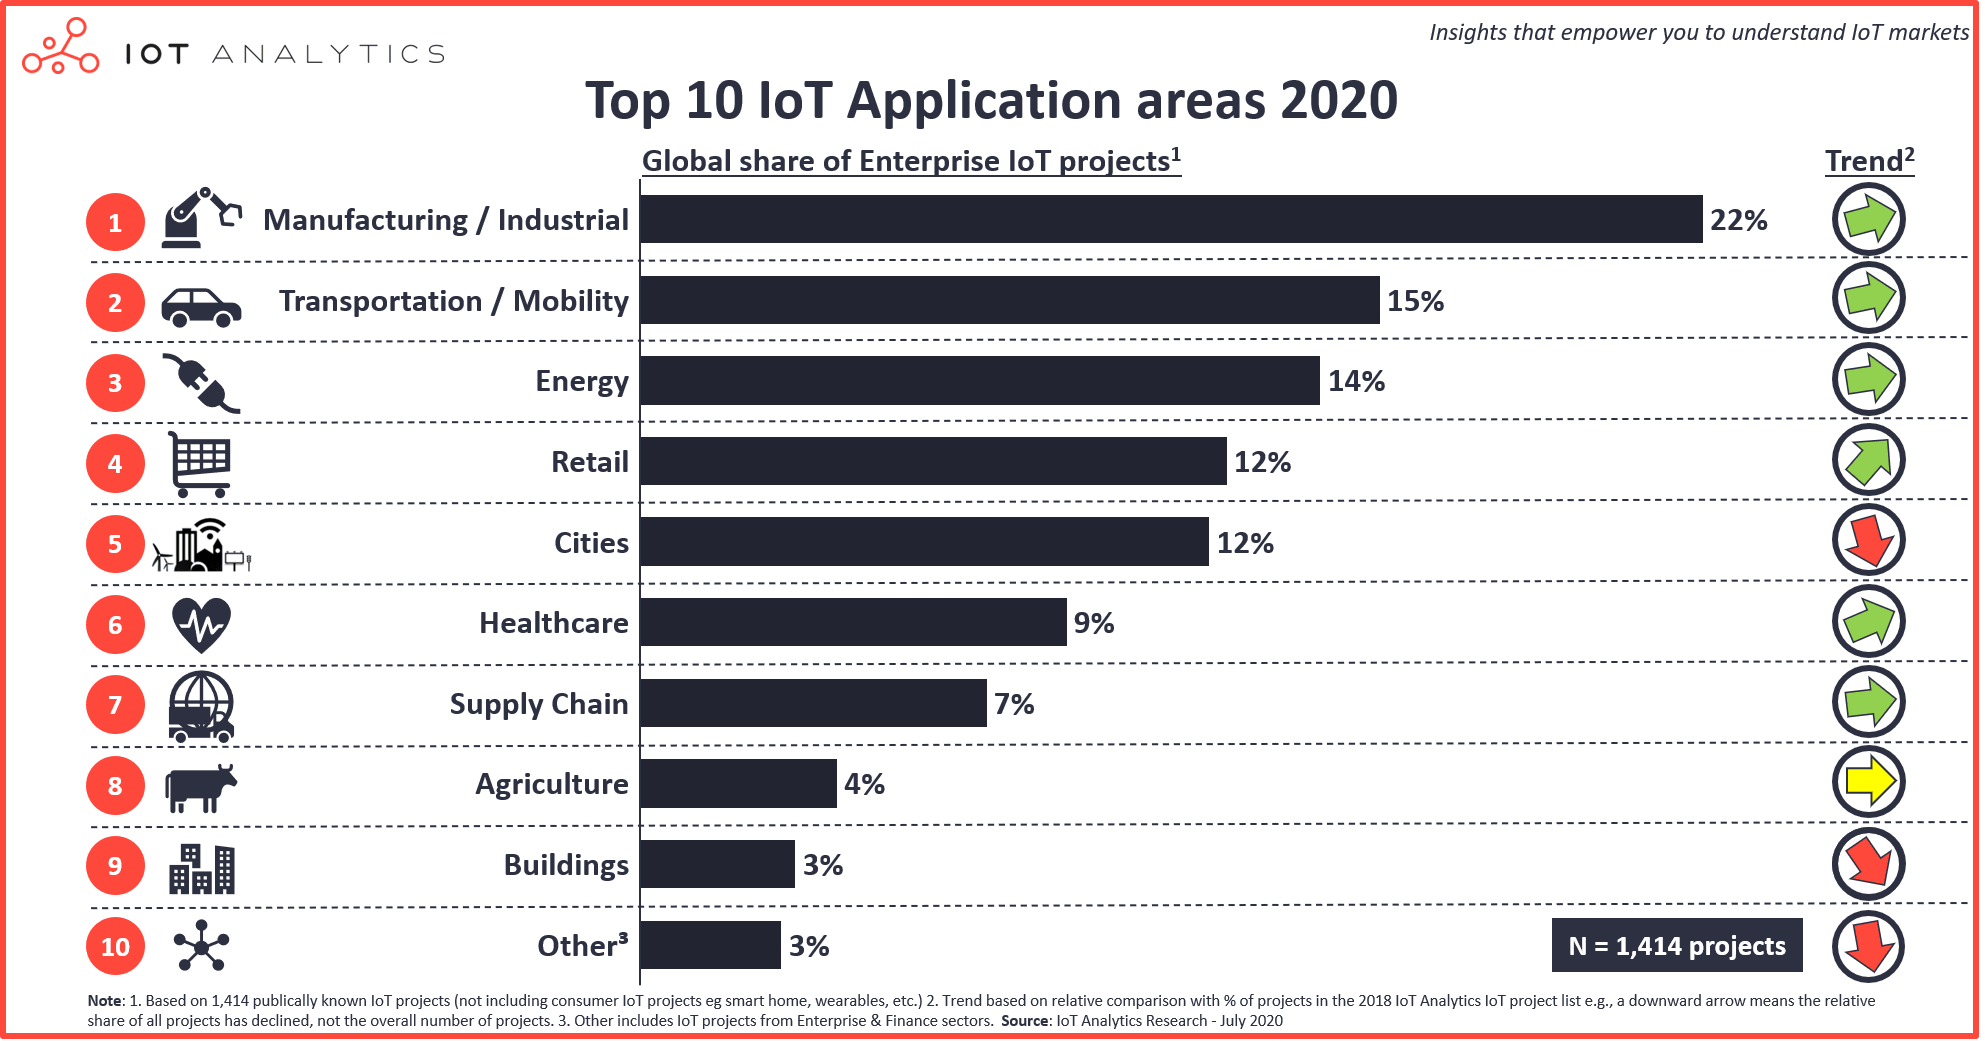
\includegraphics{images/Top-10-IoT-applications-in-2020-min.png}
\textbf{Top 10 IoT application areas}

Smart cities are the stimulus for the first discussion in the forum this week. A video clip sets out the possibilities and the pitfalls\footnote{\protect\hyperlink{china-scs}{I've already talked about this}.}.

\hypertarget{activity-what-do-you-think-are-the-biggest-concerns-raised-by-the-internet-of-things}{%
\subsection{Activity: what do you think are the biggest concerns raised by the Internet of Things?}\label{activity-what-do-you-think-are-the-biggest-concerns-raised-by-the-internet-of-things}}

For me, there is clearly the potential for the abuse of power. Surveillance by digital means is less visible but no less terrifying than Goebbels' yellow badge.

\hypertarget{hammer-chewers}{%
\subsection{Hammer Chewers}\label{hammer-chewers}}

A further video introduces further the IoT using a ``two people pretend to interview each other'' approach which is a bit cheesy, especially as neither are natural presenters. I'm finding the pedagogy of this course fascinating: for a University which has a School of Education, it's eye-rolling (face-palming?) to see academics who think they know how to teach, actually try. To be fair, it's not unique to Edinburgh: this problem presents itself in other courses I have seen. It's a delighfully ironic example of Dunning-Krueger (Kruger \& Dunning, \protect\hyperlink{ref-Kruger1999}{1999}).

\hypertarget{so-what-is-it}{%
\subsection{So, what is it?}\label{so-what-is-it}}

Imagine the world in the age of the new telegraph. Messages can be sent from place to place, if those places are connected by wires. Add to this, the technological advances in sensing the environment, and we have \emph{telemetry}. The ability and desire to save our legs has been the driver of innovation: the \href{https://en.wikipedia.org/wiki/Trojan_Room_coffee_pot}{Trojan Room Coffee Pot} is a legendary modern example. Now, the Internet provides the wires for communication, and miniaturisation and scaling of sensors provides a deluge of data. The IoT is not a new thing at all, merely the development of something much older. It is telemetry, but with the added bonus of aggregation and inference: analysis of increasing amounts of data from the physical world yields insights we didn't have before.

What makes it interesting is the development of the neural network and the inferences they can make from many data points. Inferences that can aid policy and management decisions (like, ``do we need street lights on in this district between 2 am and 4 am?''). Inferences like ``these districts are more prone to drug crime''.

What is described as the datafication of the environment is surely an exaggeration, but the more we know about the world, then so must our choices be improved?

The problems arise when data is re-purposed. This problem is also identified as \emph{function creep}. Steps are being taken now to make it harder for this re-purposing of data to happen without the provider of the data having informed awareness, and giving their informed consent for it to be used in a new or different way than was understood. ``Doing data protection by design and default'' is mentioned in the video to suggest that limits can be placed on the use of the data when innovation is taking place.

\hypertarget{the-smart-home}{%
\section{The Smart Home}\label{the-smart-home}}

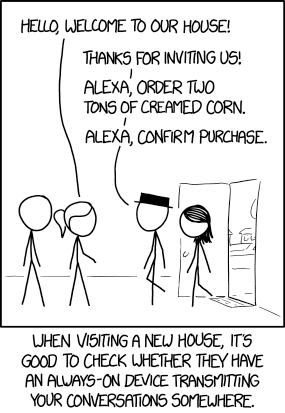
\includegraphics{images/listening.png}
Cartoon \emph{Listening} © \href{https://xkcd.com/1807/\%20\%5BCC\%20BY-NC\%202.5\%5D(https://creativecommons.org/licenses/by-nc/2.5/)}{XKCD}

The situation is set out for us: we are using technologies, sometimes without having the right to refuse, which are gathering data on us, our homes, and our lives. The ethical concerns associated with these innovations are characterised as being of two kinds: \emph{Social and cultural concerns}; and \emph{Governance concerns}.

\hypertarget{audit-and-share}{%
\subsection{Audit and share}\label{audit-and-share}}

Students on the course are invited to consider and share their thoughts on the risks and benefits of smart devices. We are challenged to consider the security measures we (may) have taken to protect privacy as we use them.

I did an audit of my home and consider it not to be so smart: we have wifi, of course, with an up to date firewall and port management; an Amazon Fire Stick on one of the stupid TVs to make it smarter; an Amazon Echo Dot that is just hilarious\footnote{Try the extreme farts extension pack for Alexa.}, that we got free with the Hive device for the boiler.

\hypertarget{governance}{%
\subsection{Governance}\label{governance}}

Laws like GDPR address concerns like \emph{opaque data flows}, where data is moved around and shared within systems without the awareness of the people using those systems. These laws try to ensure that users are informed about these data flows and have some sense of choice, although it is evident that these mechanisms fail: they are themselves opaque and inaccessible to users. A modern defence is obfuscation -- burying it with bureaucracy -- and one which organisations use extensively to hold up a veil of compliance and transfer blame to the participants or users who are too lazy to fill the forms in, or read the Ts \& Cs\footnote{This particular problem is causing me considerable difficulty at the moment. Systems purported to support staff and students are in fact stressors because they present a wall of undifferentiated administration where none is required, or at least, a minimal set and some principles that, once clearly stated, are all those staff and students need to decide for themselves how to comply with requirements. It's incompetence but because it is presented as ``action in support'', nothing is done about it and those who speak out are seen to be oppugnant. One has empathy with \href{https://en.wikipedia.org/wiki/John_Grigg_(writer)}{Lord Altrincham}.}.

Academics write that privacy involves protecting the \emph{context} of data as much as the data itself.

\hypertarget{examples-activity}{%
\subsection{Examples activity}\label{examples-activity}}

We are encouraged to ``share and comment'' on a \href{https://padlet.com/moocdeliveryteam/m6er1x8gmb8t6b2j}{Padlet} articles relating to four examples: internet-connected home systems; smart homes for the elderly; Alexa/Echo; and smart meters\footnote{Apart from my hatred of Padlet and similar ``digital equivalents to something useful'', I am too short of time for this. The time estimate for this course is way off the 3 hours a week for a full engagement with it and I am a little frustrated by not being able to dive into the wider reading. I really wanted to look at Danah Boyd's paper on teenagers' engagement with technology but that will have to just pass me by. This is not a criticism of the course, but of my own stupidity in engaging with it at this time.}.

\hypertarget{references}{%
\chapter*{References}\label{references}}
\addcontentsline{toc}{chapter}{References}

\hypertarget{refs}{}
\begin{cslreferences}
\leavevmode\hypertarget{ref-asimov1991foundation}{}%
Asimov, I. (1991). \emph{Foundation}. Bantam Books.

\leavevmode\hypertarget{ref-Bardi2018}{}%
Bardi, A., Holloway, R., Lönnqvist, J.-E., Bevington, P., Hanel, P. H. P., Maio, G. R., Soares, A. K. S., Vione, K. C., De Holanda Coelho, G. L., Gouveia, V. V., Patil, A. C., Kamble, S. V., \& Manstead, A. S. R. (2018). \emph{Cross-Cultural Differences and Similarities in Human Value Instantiation}. \url{https://doi.org/10.3389/fpsyg.2018.00849}

\leavevmode\hypertarget{ref-Barocas2014}{}%
Barocas, S. (2014). Big Data's Disparate Impact. \emph{California Law Review}, \emph{104}(671), 671--732.

\leavevmode\hypertarget{ref-OED-bias}{}%
\emph{bias, adj., n., and adv. : Oxford English Dictionary}. (n.d.). Retrieved November 16, 2020, from \url{https://www.oed.com/view/Entry/18564?result=1\&rskey=pOoRi9\&}

\leavevmode\hypertarget{ref-TitleVii1964}{}%
\emph{Civil Rights Act of 1964 - CRA - Title VII - Equal Employment Opportunities - 42 US Code Chapter 21}. (1964). \url{https://finduslaw.com/civil-rights-act-1964-cra-title-vii-equal-employment-opportunities-42-us-code-chapter-21}

\leavevmode\hypertarget{ref-Contreras2019}{}%
Contreras, D. V. (2019). \emph{Batallas 3.0: Inteligencia Artificial y algoritmos versus delincuencia en Chile}. \url{https://www.theclinic.cl/2019/07/25/batallas-3-0-inteligencia-artificial-y-algoritmos-versus-delincuencia-en-chile/}

\leavevmode\hypertarget{ref-Couchman2019}{}%
Couchman, H. (2019). \emph{Policing by Machine} (pp. 1--48). Liberty.

\leavevmode\hypertarget{ref-Ferguson2017}{}%
Ferguson, A. G. (2017). Predictive policing. \emph{Washington University Law Review}, \emph{94}(5), 1109--1189.

\leavevmode\hypertarget{ref-Goldsman2019}{}%
Goldsman, A. (2019). \emph{"Star Trek: Discovery" Context Is for Kings (TV Episode 2017)}. CBS Television Studios. \url{https://www.imdb.com/title/tt5835714/?ref_=ttep_ep3}

\leavevmode\hypertarget{ref-Huxley1955}{}%
Huxley, A. (1955). \emph{Brave new world : a novel}. Penguin Books in association with Chatto \& Windus.

\leavevmode\hypertarget{ref-IoTAnalytics2020}{}%
IoT Analytics. (2020). \emph{Top 10 IoT applications in 2020 - Which are the hottest areas right now?} \url{https://iot-analytics.com/top-10-iot-applications-in-2020/}

\leavevmode\hypertarget{ref-Kirkpatrick2016}{}%
Kirkpatrick, K. (2016). Battling algorithmic bias. \emph{Communications of the ACM}, \emph{59}(10), 16--17. \url{https://doi.org/10.1145/2983270}

\leavevmode\hypertarget{ref-Kruger1999}{}%
Kruger, J., \& Dunning, D. (1999). Unskilled and unaware of it: How difficulties in recognizing one's own incompetence lead to inflated self-assessments. \emph{Journal of Personality and Social Psychology}, \emph{77}(6), 1121--1134. \url{https://doi.org/10.1037/0022-3514.77.6.1121}

\leavevmode\hypertarget{ref-Shakespeare}{}%
Shakespeare, W. (1591). \emph{Henry VI, part 2: Entire Play}. \url{http://shakespeare.mit.edu/2henryvi/full.html}

\leavevmode\hypertarget{ref-Taylor2017}{}%
Taylor, L. (2017). What is data justice? The case for connecting digital rights and freedoms globally. \emph{Big Data and Society}, \emph{4}(2), 1--14. \url{https://doi.org/10.1177/2053951717736335}

\leavevmode\hypertarget{ref-Tolan2018}{}%
Tolan, S. (2018). \emph{JRC Digital Economy Working Paper 2018-10 Fair and Unbiased Algorithmic Decision Making : Current State and Future Challenges}. \emph{December}.

\leavevmode\hypertarget{ref-TURING1950}{}%
Turing, A. M. (1950). Computing Machinery and Intelligence. \emph{Mind}, \emph{LIX}(236), 433--460. \url{https://doi.org/10.1093/mind/LIX.236.433}

\leavevmode\hypertarget{ref-Hildebrandt2019}{}%
Wagner, B. (2019). Ethics As An Escape From Regulation. From ``Ethics-Washing'' To Ethics-Shopping? In M. Hildebrandt (Ed.), \emph{Being profiled} (pp. 84--89). \url{https://doi.org/10.1515/9789048550180-016}
\end{cslreferences}

\end{document}
